\begin{frame}{Encoder-Decoder Architecture}
  \begin{itemize}
    \item[\textcolor{red}{$\blacktriangleright$}] \textbf{Encoder:} Stack of self-attention and feed-forward (FF) layers.
    \item[\textcolor{red}{$\blacktriangleright$}] \textbf{Decoder:} Adds masked self-attention and encoder-decoder attention on top of FF layers.
    \item[\textcolor{red}{$\blacktriangleright$}] \textbf{Applications:} Widely used in tasks like translation, summarization, and more.
  \end{itemize}
\end{frame}

\begin{frame}{Encoder}
  \centering
  
\includegraphics[width=\paperwidth,height=0.95\paperheight,keepaspectratio]{assets/Lecture-6_Introduction_to_Transformers/pdf_page_056.png}
\end{frame}

\begin{frame}{Encoder}
  \centering
  
\includegraphics[width=\paperwidth,height=0.95\paperheight,keepaspectratio]{assets/Lecture-6_Introduction_to_Transformers/pdf_page_057.png}
\end{frame}

\begin{frame}{Encoder}
  \centering
  
\includegraphics[width=\paperwidth,height=0.95\paperheight,keepaspectratio]{assets/Lecture-6_Introduction_to_Transformers/pdf_page_058.png}
\end{frame}

\begin{frame}{Encoder}
  \centering
  
\includegraphics[width=\paperwidth,height=0.95\paperheight,keepaspectratio]{assets/Lecture-6_Introduction_to_Transformers/pdf_page_059.png}
\end{frame}

\begin{frame}{Encoder}
  \centering
  
\includegraphics[width=\paperwidth,height=0.95\paperheight,keepaspectratio]{assets/Lecture-6_Introduction_to_Transformers/pdf_page_060.png}
\end{frame}

\begin{frame}{Encoder-Only Transformers}
  \begin{itemize}
    \item[\textcolor{red}{$\blacktriangleright$}] \textbf{Example:} BERT
    \item[\textcolor{red}{$\blacktriangleright$}] Only the encoder stack is used.
    \item[\textcolor{red}{$\blacktriangleright$}] \textbf{Applications:} Classification, question answering, embeddings.
  \end{itemize}
\end{frame}

\begin{frame}{Encoders}
  \centering
  
\includegraphics[width=0.8\paperwidth,height=0.8\paperheight,keepaspectratio]{assets/Lecture-6_Introduction_to_Transformers/pdf_page_062.png}
\end{frame}

\begin{frame}{Encoders}
  \centering
  
\includegraphics[width=0.8\paperwidth,height=0.8\paperheight,keepaspectratio]{assets/Lecture-6_Introduction_to_Transformers/pdf_page_063.png}
\end{frame}

\begin{frame}{Encoder-Decoder Attention}
  \centering
  
\includegraphics[width=0.9\paperwidth,height=0.9\paperheight,keepaspectratio]{assets/Lecture-6_Introduction_to_Transformers/pdf_page_064.png}
\end{frame}

\begin{frame}{Encoder-Decoder Attention}
  \centering
    
\includegraphics[width=0.9\paperwidth,height=0.9\paperheight,keepaspectratio]{assets/Lecture-6_Introduction_to_Transformers/pdf_page_065.png}
\end{frame}

\begin{frame}{Encoder-Decoder Attention}
  \centering
  
\includegraphics[width=0.9\paperwidth,height=0.9\paperheight,keepaspectratio]{assets/Lecture-6_Introduction_to_Transformers/pdf_page_066.png} 
\end{frame}

\begin{frame}{Encoder-Decoder Attention}
  \centering
  
\includegraphics[width=0.9\paperwidth,height=0.9\paperheight,keepaspectratio]{assets/Lecture-6_Introduction_to_Transformers/pdf_page_067.png}
\end{frame}

\begin{frame}{Encoder-Decoder Attention}
  \centering
  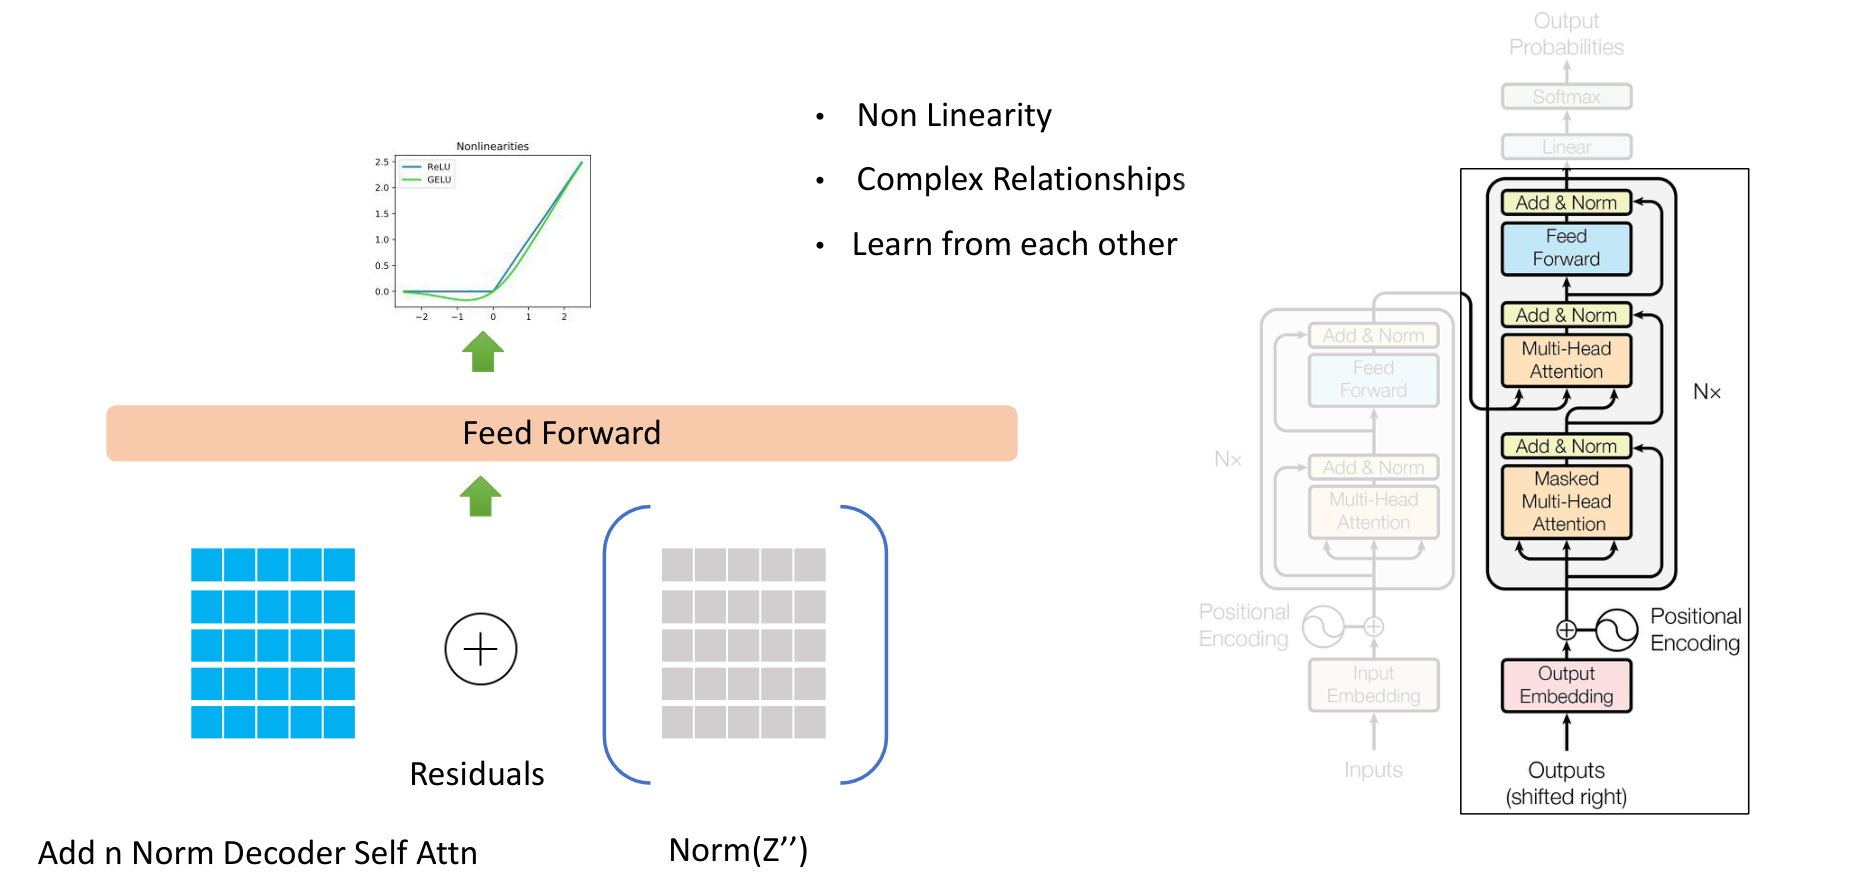
\includegraphics[width=0.9\paperwidth,height=0.9\paperheight,keepaspectratio]{assets/Lecture-6_Introduction_to_Transformers/pdf_page_068.png}
\end{frame}

\begin{frame}{Decoder-Only Transformers}
  \begin{itemize}
    \item[\textcolor{red}{$\blacktriangleright$}] \textbf{Example:} GPT, LLaMA
    \item[\textcolor{red}{$\blacktriangleright$}] Uses only the decoder block.
    \item[\textcolor{red}{$\blacktriangleright$}] \textbf{Masked self-attention (causal):} Each token can only attend to previous tokens.
    \item[\textcolor{red}{$\blacktriangleright$}] \textbf{Applications:} Language modeling, text generation.
  \end{itemize}
\end{frame}

\begin{frame}{Decoder}
  \centering
  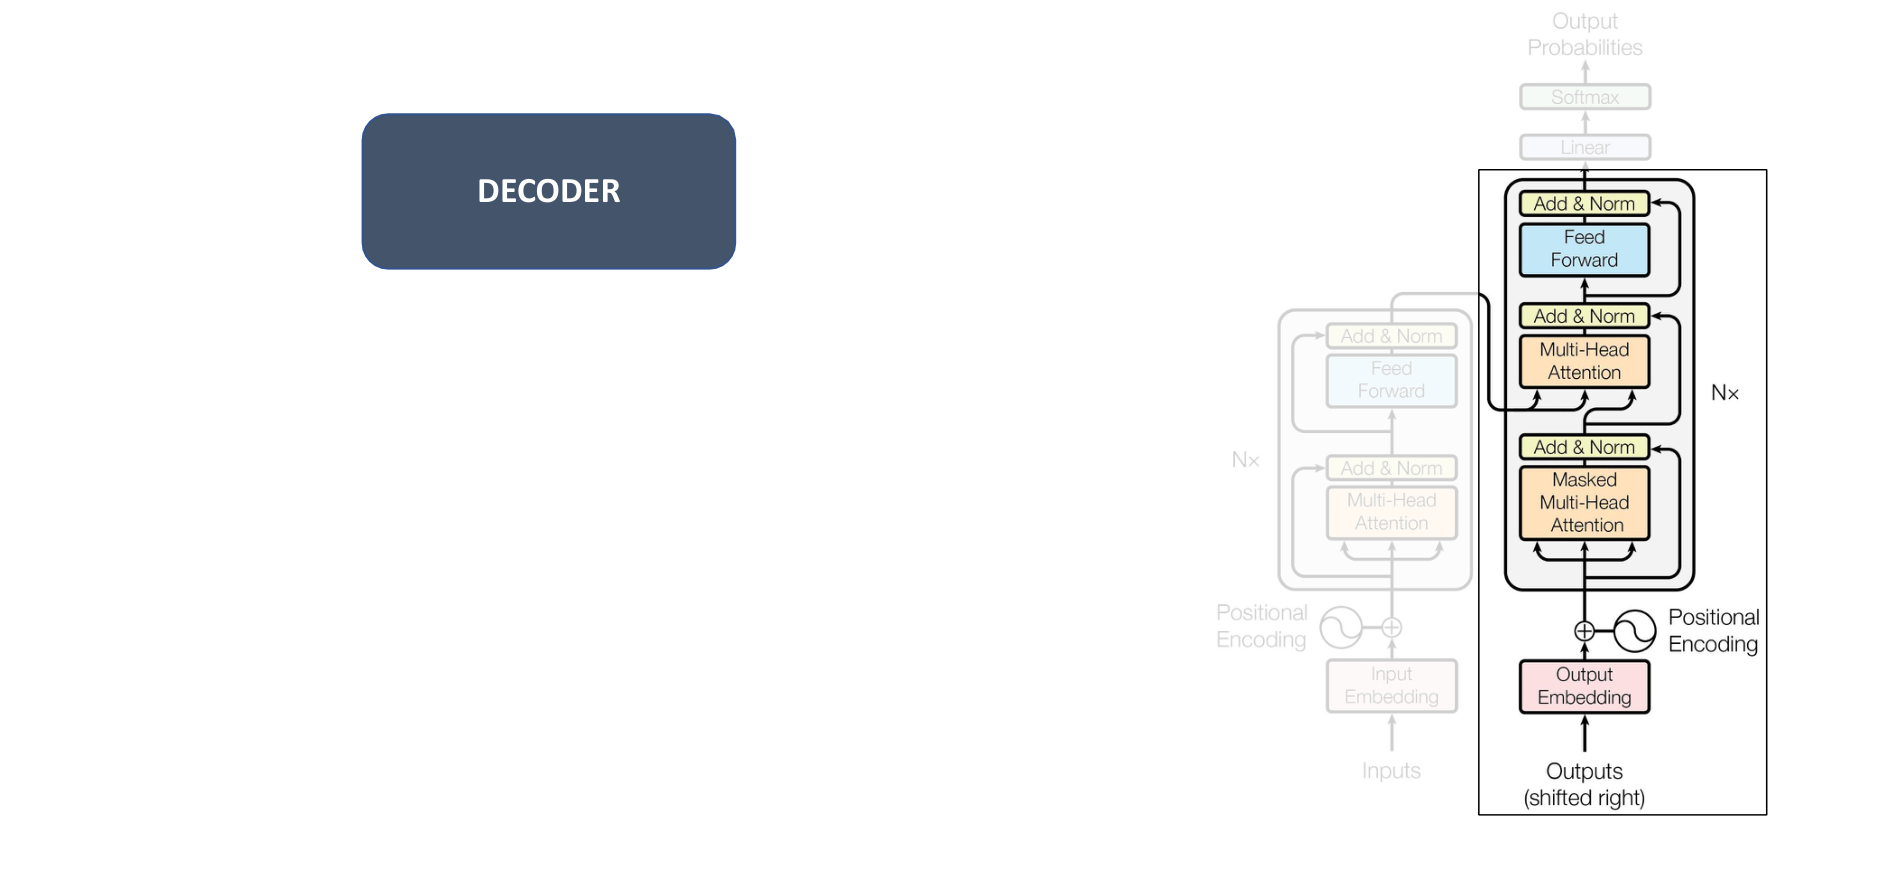
\includegraphics[width=0.8\paperwidth,height=0.8\paperheight,keepaspectratio]{assets/Lecture-6_Introduction_to_Transformers/pdf_page_070.png}
\end{frame}

\begin{frame}{Decoder}
  \centering
  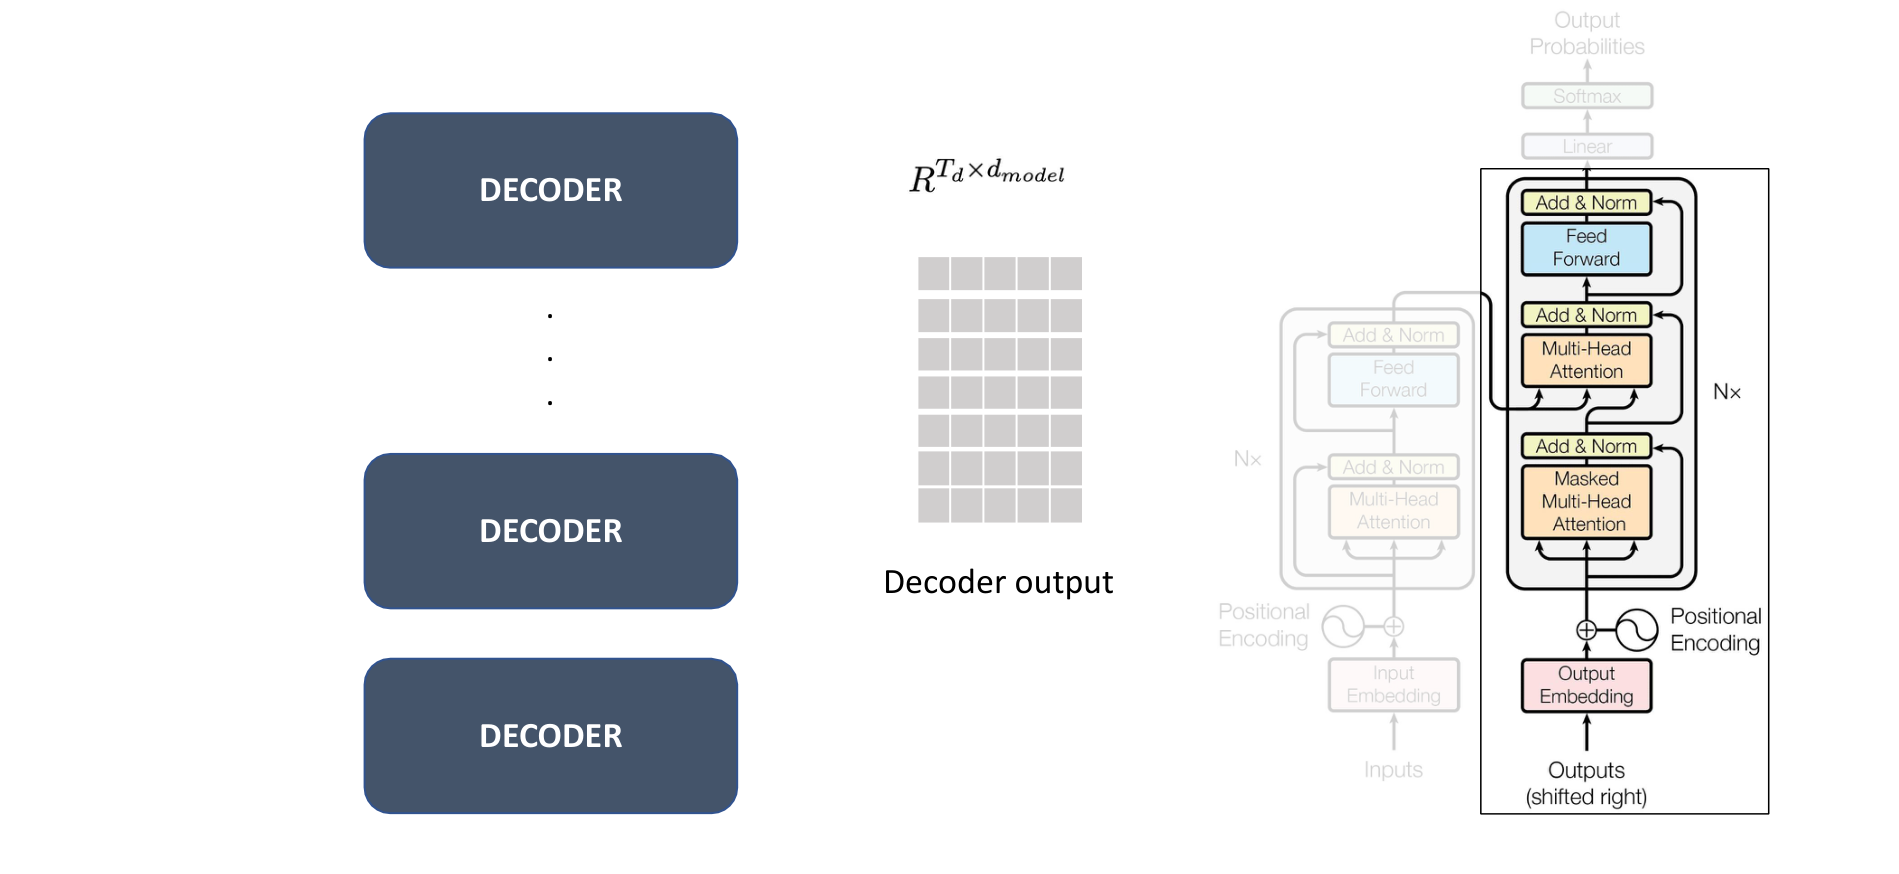
\includegraphics[width=0.8\paperwidth,height=0.8\paperheight,keepaspectratio]{assets/Lecture-6_Introduction_to_Transformers/pdf_page_071.png}
\end{frame}

\begin{frame}{Linear}
  \centering
  
\includegraphics[width=0.8\paperwidth,height=0.8\paperheight,keepaspectratio]{assets/Lecture-6_Introduction_to_Transformers/pdf_page_072.png}
\end{frame}

\begin{frame}{Softmax}
  \centering
  
\includegraphics[width=0.8\paperwidth,height=0.8\paperheight,keepaspectratio]{assets/Lecture-6_Introduction_to_Transformers/pdf_page_073.png}
\end{frame}

\begin{frame}{Transformers}
  \centering
  
\includegraphics[width=0.9\paperwidth,height=0.9\paperheight,keepaspectratio]{assets/Lecture-6_Introduction_to_Transformers/pdf_page_074.png}
\end{frame}

\begin{frame}{Transformers}
  \centering
  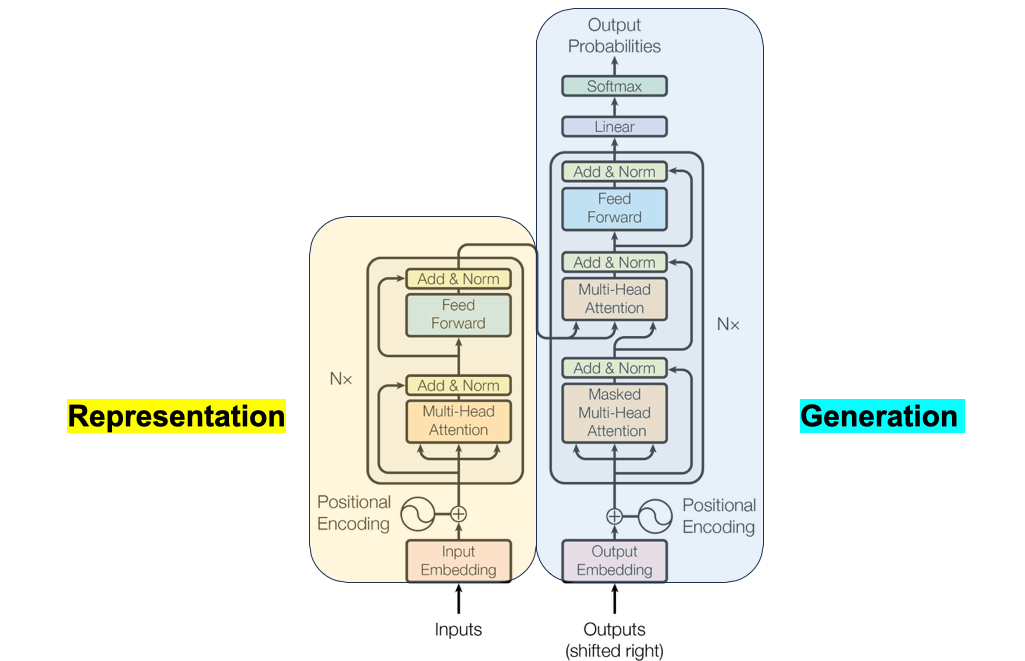
\includegraphics[width=0.8\paperwidth,height=0.8\paperheight,keepaspectratio]{assets/Lecture-6_Introduction_to_Transformers/pdf_page_075.png}
\end{frame}

\begin{frame}{Transformers}
  \centering
  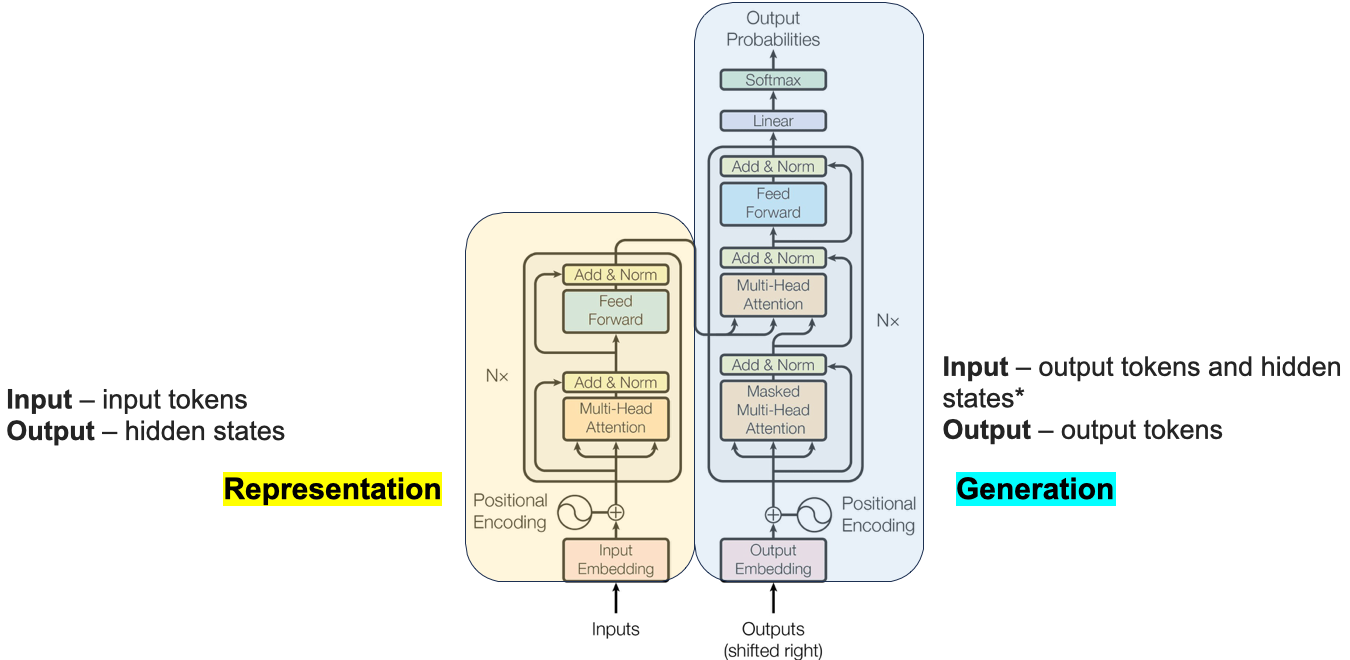
\includegraphics[width=0.9\paperwidth,height=0.9\paperheight,keepaspectratio]{assets/Lecture-6_Introduction_to_Transformers/pdf_page_076.png}
\end{frame}

\begin{frame}{Transformers}
  \centering
  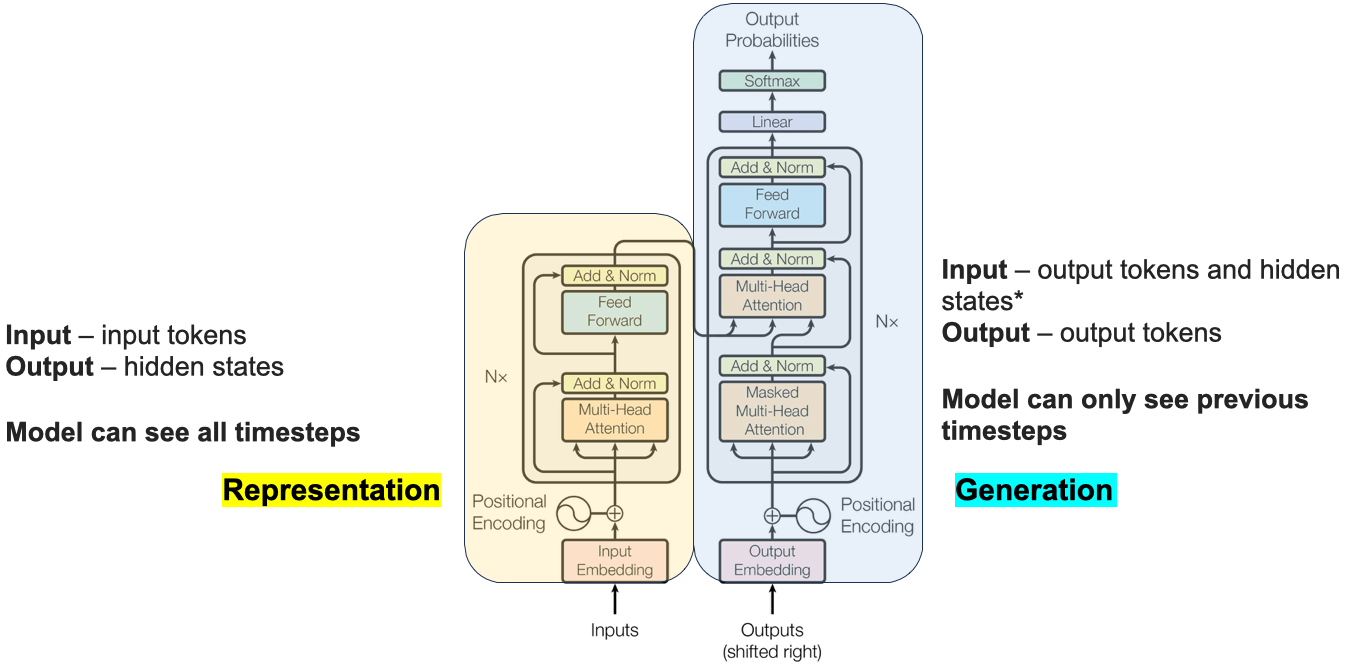
\includegraphics[width=0.8\paperwidth,height=0.8\paperheight,keepaspectratio]{assets/Lecture-6_Introduction_to_Transformers/pdf_page_077.png}
\end{frame}

\begin{frame}{Transformers}
  \centering
  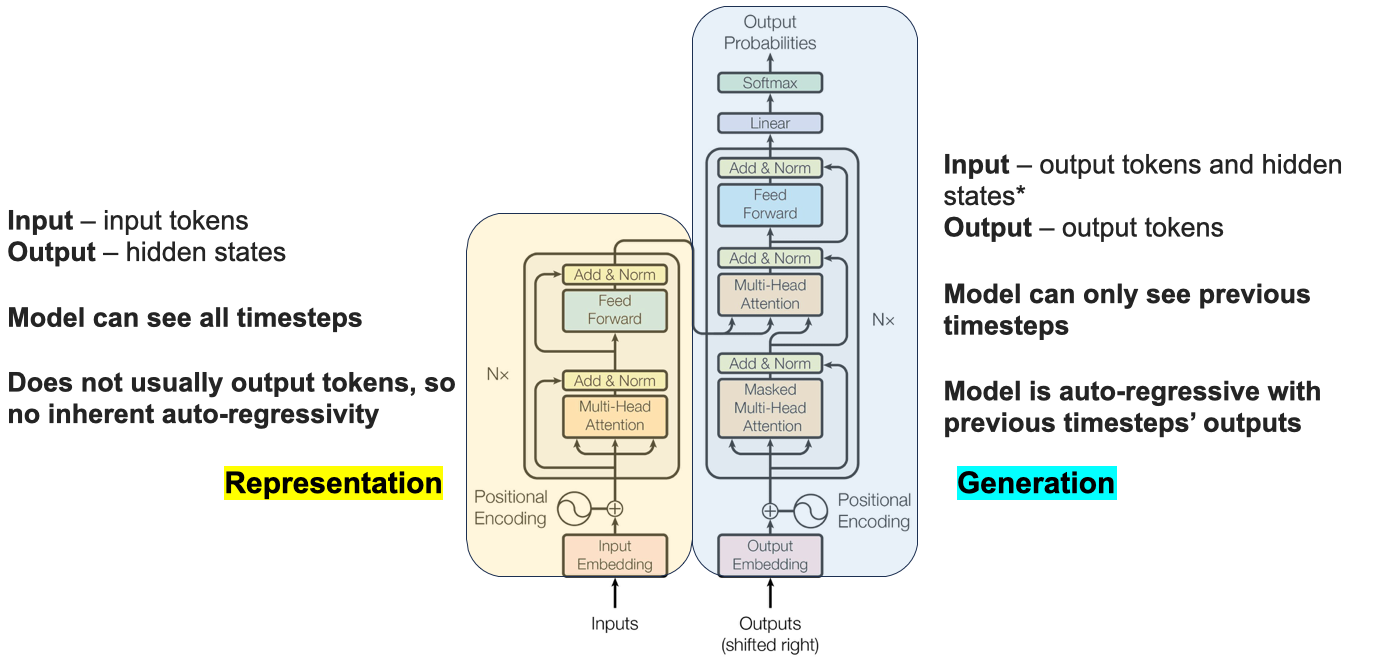
\includegraphics[width=0.8\paperwidth,height=0.8\paperheight,keepaspectratio]{assets/Lecture-6_Introduction_to_Transformers/pdf_page_078.png}
\end{frame}

\begin{frame}{Transformers}
  \centering
  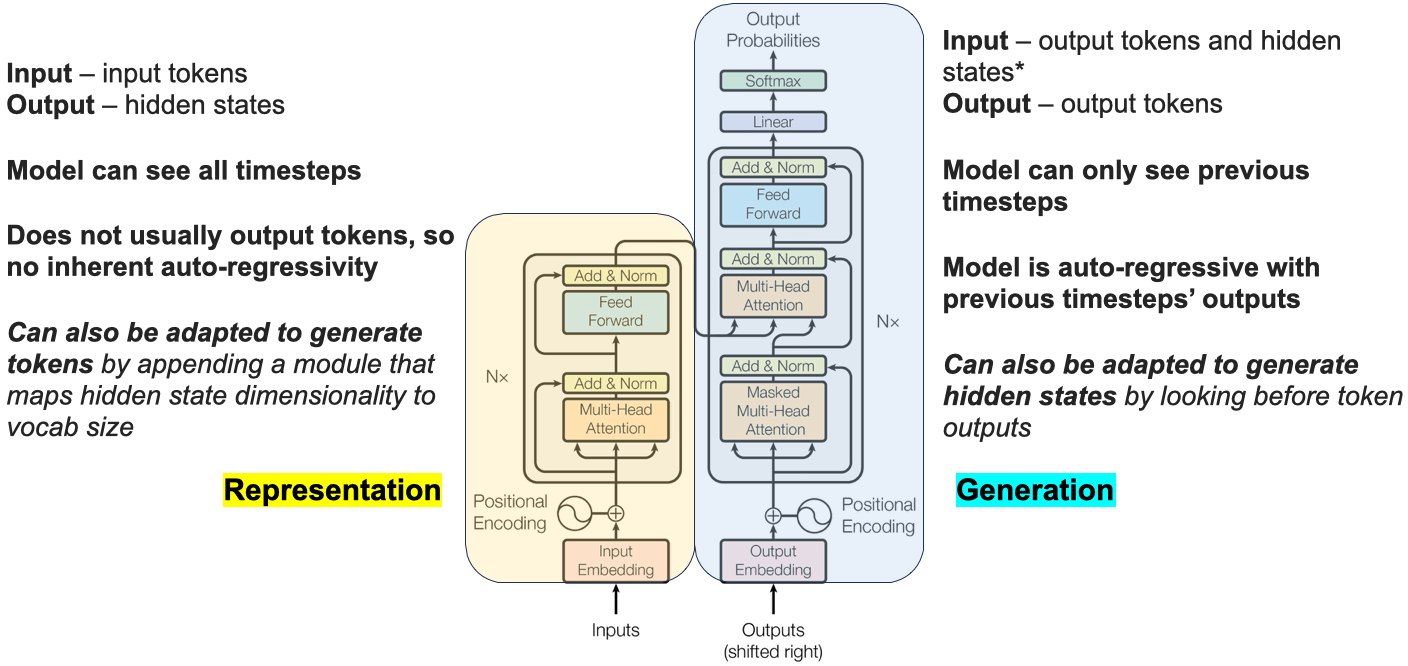
\includegraphics[width=0.8\paperwidth,height=0.8\paperheight,keepaspectratio]{assets/Lecture-6_Introduction_to_Transformers/pdf_page_079.png}
\end{frame}

